\documentclass[12pt,twoside]{article}
\usepackage[utf8]{inputenc}
\usepackage[usenames]{xcolor}
\newcommand{\alert}[1]{{\color{red}#1}}
\usepackage{cancel}
\usepackage{answers}
\usepackage{centernot}
\usepackage{setspace}
\usepackage{graphicx}
\usepackage{enumerate}
\usepackage{multicol}
\usepackage[margin=0.7in]{geometry} 
\usepackage{amsmath,amsthm,amssymb}
\usepackage[none]{hyphenat}
\usepackage{fancyhdr} 
\usepackage{wasysym}
\usepackage[rightcaption]{sidecap}
\usepackage{amsmath}
\usepackage{wrapfig} %insertar figuras en cualquier parte de la página
\usepackage{imakeidx}
\usepackage[framemethod=tikz]{mdframed}
\usepackage[breakable,most]{tcolorbox}

\usepackage{tikz}
\usetikzlibrary{positioning}
\usetikzlibrary{shadows} %shadedbox

\usepackage [english]{babel}
\usepackage [autostyle, english = american]{csquotes}
\MakeOuterQuote{"}

\usepackage{titlesec}
\usepackage{lipsum} %texto genérico
\usepackage[colorlinks=true,linkcolor=black]{hyperref} %links de índice
\usepackage{tikz}
\usepackage{yhmath}
\usepackage{mathdots}
\usepackage{cleveref}
\usepackage{epstopdf}
\usepackage{mathrsfs}

\usepackage{algorithm}
\usepackage{algpseudocode}


\epstopdfDeclareGraphicsRule{.gif}{png}{.png}{convert gif:#1 png:\OutputFile}
\AppendGraphicsExtensions{.gif}


\usepackage{pgfplots,tikz}
\usepgfplotslibrary{fillbetween}
\usetikzlibrary {arrows.meta}
\usepackage{circuitikz}
\usetikzlibrary{decorations.markings}
\usepackage{esint}
\pgfplotsset{width=10cm,compat=newest}
\usepgfplotslibrary{external}
\tikzexternalize

\newcommand{\N}{\mathbb{N}}
\newcommand{\Z}{\mathbb{Z}}
\newcommand{\C}{\mathbb{C}}
\newcommand{\R}{\mathbb{R}}
\newcommand{\Q}{\mathbb{Q}}
\newcommand{\p}{\mathbb{P}}
\newcommand{\K}{\mathbb{K}}
\newcommand{\ssi}{\Longleftrightarrow}
\newcommand{\longto}{\longrightarrow}
\newcommand{\Arg}{\operatorname{Arg}}
\newcommand{\cis}{\operatorname{c}\dot\imath\operatorname{s}}
\newcommand{\dom}{\operatorname{dom}}
\DeclareMathOperator{\sech}{sech}
\DeclareMathOperator{\csch}{csch}

\usepackage[shortlabels]{enumitem}


\newenvironment{definition}[2][Definici\'on]{\begin{trivlist}
		\item[\hskip \labelsep {\bfseries #1}\hskip \labelsep {\bfseries #2.}]}{\end{trivlist}}
\newenvironment{proposicion}[2][\(\blacksquare\) Proposici\'on]{\begin{trivlist}
		\item[\hskip \labelsep {\bfseries #1}\hskip \labelsep {\bfseries #2.}]}{\end{trivlist}}
\newenvironment{lemma}[2][Lemma]{\begin{trivlist}
		\item[\hskip \labelsep {\bfseries #1}\hskip \labelsep {\bfseries #2.}]}{\end{trivlist}}
\newenvironment{exercise}[2][Exercise]{\begin{trivlist}
		\item[\hskip \labelsep {\bfseries #1}\hskip \labelsep {\bfseries #2.}]}{\end{trivlist}}
\newenvironment{solution}[2][\textcolor{teal}{Solución:}]{\begin{trivlist}
		\item[\hskip \labelsep {\bfseries #1}]}{\end{trivlist}}
\newenvironment{problem}[2][\textcolor{purple}{Problema}]{\begin{trivlist}
		\item[\hskip \labelsep {\bfseries \textcolor{purple}{#1}}\hskip \labelsep {\bfseries \textcolor{purple}{#2.}}]}{\end{trivlist}}
\newenvironment{question}[2][Question]{\begin{trivlist}
		\item[\hskip \labelsep {\bfseries #1}\hskip \labelsep {\bfseries #2.}]}{\end{trivlist}}
\newenvironment{obs}[2][\textcolor{red}{Observaci\'on}]{\begin{trivlist}
		\item[\hskip \labelsep {\bfseries \textcolor{red}{#1}}\hskip \labelsep {\bfseries \textcolor{red}{#2.}}]}{\end{trivlist}}


\fancypagestyle{plain}{
	
	\fancyhead[LE,RO]{\includegraphics[scale=0.074]{Isotipo-Negro.png}} %inserta logo de la u, width es tamaño de la imagen
	\fancyhead[LO,RE]{\begin{footnotesize}\normalsize{\textsc{Universidad Técnica Federico Santa María\\Departamento de Matemática\\MAT282 \textthreequartersemdash\ Laboratorio de Modelaci\'on \\ Segundo Semestre 2023}}\end{footnotesize}}
	\fancyfoot[CE,CO]{\begin{footnotesize} \end{footnotesize}}
	\fancyfoot[LE,RO]{\begin{footnotesize}\thepage\end{footnotesize}}
	\renewcommand{\headrulewidth}{1pt}
	\renewcommand{\footrulewidth}{0.4pt}
}
\setlength{\headheight}{61pt}
\setlength{\textheight}{650pt}
\pagestyle{plain}


\usepackage{listings}
\allowdisplaybreaks
%\usepackage{courier}
\definecolor{codegreen}{rgb}{0,0.6,0}
\definecolor{codegray}{rgb}{0.5,0.5,0.5}
\definecolor{codepurple}{rgb}{0.58,0,0.82}
\definecolor{backcolour}{rgb}{0.95,0.95,0.92}

\lstdefinestyle{mystyle}{
	backgroundcolor=\color{backcolour},   
	commentstyle=\color{codegreen},
	keywordstyle=\color{magenta},
	numberstyle=\tiny\color{codegray},
	stringstyle=\color{codepurple},
	basicstyle=\ttfamily\footnotesize,
	breakatwhitespace=false,         
	breaklines=true,                 
	captionpos=b,                    
	keepspaces=true,                 
	numbers=left,                    
	numbersep=5pt,                  
	showspaces=false,                
	showstringspaces=false,
	showtabs=false,                  
	tabsize=2
}

\lstset{style=mystyle}

\title{\textbf{\textcolor{blue}{MAT282 \textthreequartersemdash\ Laboratorio de Modelaci\'on }}\color{gray} \\ Optimizaci\'on y visualizaci\'on de la planificaci\'on \'optima de una red el\'ectrica de tres nodos a lo largo de un d\'ia}
\author{\begin{tabular}{rl}
		\textbf{Profesor:} & Julio Deride.\\
		\textbf{Especialista:} & Nicol\'as Hern\'andez. \\
		\textbf{Alumnos:} & Vicente Moreno, \\
		& Martina Blanco.
\end{tabular}}
\date{}

\usepackage{parskip}


\begin{document}
	
	\maketitle
	\color{black}
	
	\newpage
	
	\renewcommand\contentsname{Indice}
	\tableofcontents

	
	\newpage
	
	\section{Introducci\'on al problema}
	
	\hspace{1cm} En la sociedad actual, una problem\'atica que tiene que resolver cada pa\'is, ciudad o pueblo es la forma de obtener energía el\'ectrica de la manera más económica pero sustentable posible. Cada una de estas ubicaciones tiene su propia producci\'on el\'ectrica y demandas que satisfacer a lo largo de un d\'ia. Adem\'as, estas ubicaciones pueden interactuar entre s\'i en una red el\'ectrica, enviando y/o recibiendo flujo el\'ectrico. Como en cada zona hay distintas demandas, producciones internas, costo de producci\'on de energ\'ia el\'ectrica y hay p\'erdidas asociadas al transmitir energ\'ia, es complicado coordinar todas las ubicaci\'ones para minimizar el costo total de la red el\'ectrica completa. Este trabajo resuelve esta problem\'atica en una red el\'ectrica reducida a tres ubicaciones, que tienen su propia producci\'on el\'ectrica y demandas que satisfacer, inspirada en la red el\'ectrica de Chile.
	
	El objetivo principal de este trabajo es modelar la red el\'ectrica chilena a lo largo de un d\'ia, para obtener una planificaci\'on a realizar para satisfacer las demandas al menor costo posible. Para esto, se consideraron como los tres agentes principales en la red el\'ectrica chilena el Norte, Centro y Sur de Chile, donde cada una de estas zonas se le asignaron producci\'ones y demandas de energ\'ia el\'ectrica basados en datos reales. Un factor considerado en este trabajo son las diversas tecnolog\'ias productoras de energía presentes en cada una de estas zonas. Adem\'as, se diferenciaron las tecnolog\'ias presentes en cada zona de acuerdo al recurso medioambiental que utilizan para generar energ\'ia el\'ectrica, donde distinguimos las tecnolog\'ias solares, en base de carb\'on y en base de gas.
	
	Para lograr este objetivo, se desarroll\'o un c\'odigo en Python que resuelve este problema y entrega, mediante gr\'aficos y datos, informaci\'on relevante para la planificaci\'on \'optima de la red durante el d\'ia. Este c\'odigo esta basado en un algoritmo que fue modelado matemáticamente, y demostrado a ser un algoritmo muy r\'apido que encuentra una soluci\'on \'optima de este problema. Para poder aplicar este modelo a este algoritmo, se asumi\'o linealidad en trozos de las funciones de costo y de las p\'erdidas en cada flujo. Adem\'as, se modelaron diversos factores basados en datos p\'ublicos de la red el\'ectrica chilena, tales como: los costos de producir energ\'ia, las tecnolog\'ias productoras de energ\'ia, las pérdidas sujetas a cada flujo, y las demandas y capacidad de producción en cada zona.
	
	Con este c\'odigo y modelo, se realiz\'o una simulaci\'on de la red el\'ectrica chilena a lo largo de un d\'ia, resolviendo la problem\'atica cada 5 minutos desde las 0:00 hasta las 23:55. Los resultados del modelamiento se acercan al comportamiento de la vida real de esta red, como los flujos principales utilizados y las zonas con mayor tendencia a recibir y/o enviar energ\'ia. Adem\'as, por el enfoque en implementar el algoritmo previamente mencionado, el programa logra construir la planificaci\'on a lo largo del d\'ia y entregar datos num\'ericos casi instant\'aneamente.
	
	La motivación para el desarrollo de este trabajo es la visualizaci\'on de la información sobre la producción y la demanda de la energía eléctrica, y el an\'alisis que es posible extraer de las soluciones gr\'aficas de este problema. Además, aunque este trabajo est\'a centrado en analizar la red el\'ectrica chilena, es aplicable para cualquier red el\'ectrica de tres nodos. El c\'odigo en Python creado en este trabajo considera la posibilidad de ser aplicado en otros contextos, y trata de facilitar el uso de modelos distintos al considerado.
	
	\textbf{Comparaci\'on con la literatura:} En la tesis \textit{Estudio de Problemas de Optimizaci\'on y Equilibrio sobre una Red de Producci\'on El\'ectrica}, se estudia la red el\'ectrica que se plantea en este trabajo y se plantea el algoritmo ocupado en este proyecto, tambi\'en basandose en la red el\'ectrica chilena. Adem\'as, la tesis profundiza en variantes del problema de tres nodos, a\~{n}adiendo nodos satelitales a los tres nodos principales, tambi\'en describiendo un algoritmo de resolucion general para estos problemas.
	
	Los datos para modelar las demandas en cada zona, el aporte de cada tecnolog\'ia en cada zona y las funciones de costo est\'an basadas en un ejemplo explicito de la red el\'ectrica chilena del art\'iculo \textit{Pollution Regulation for Electricity Generators in a Transmission Network}, donde se estudia el problema de la red el\'ectrica como un juego estoc\'astico diferencial de Stackelberg en tiempo continuo.

	\section{Teor\'ia matem\'atica del problema}
	\subsection{Definici\'on matem\'atica del problema}
	
	\hspace{1cm} Para poder definir el problema de producci\'on en una red el\'ectrica, se necesita un conjunto finito no vac\'io que va a representar las ubicaciones que necesitan ser abastecidas con energ\'ia. Este conjunto se puede representar como nodos en un grafo dirigido, y lo llamaremos \(I\). Adem\'as, se necesita un conjunto que liste todas las posibles direcciones de env\'io entre nodos. Este conjunto se puede representar en un grafo como todos los arcos dirigidos entre nodos de \(I\), que llamaremos \(E\).
	
	\hspace{1cm} A cada nodo \(i\in I\) se le puede asignar un l\'imite de producci\'on de energ\'ia y una demanda a satisfacer, que se denominaran \(Q_i\) y \(D_i\) respectivamente. Adem\'as, es \'util considerar la colecci\'on de todos los arcos entrantes y todos los arcos salientes del nodo \(i\), que denominaran \(E_i\) y \(S_i\) respectivamente.
	
	\hspace{1cm} Las variables que se quieren obtener para resolver este problema son la producci\'on en cada nodo \(i\in I\), y los flujos de energ\'ia que transmitir entre nodos para cada conexi\'on \(j\in E\). Estas variables ser\'an \(q_i\) y \(\phi_j\) respectivamente, y la agrupaci\'on de estos se denotar\'a \((q,\phi)\). En el grafo, se puede asociar directamente a \(q_i\) con su nodo respectivo y a \(\phi_j\) a su arco respectivo.
	
	\hspace{1cm} Finalmente, se necesitan funciones que representen el costo de producci\'on y p\'erdida de env\'io. Primero, para cada nodo \(i\in I\) se define como el \textbf{costo asociado a la producci\'on de energ\'ia en un nodo} como \(\operatorname{c}_i:[0,\infty)\to[0,\infty)\). Esta funci\'on recibe una producci\'on \(q_i\) y entrega un valor monetario asociado. Adem\'as, se define la \textbf{funci\'on de p\'erdida} como \(\operatorname{r}:[0,\infty)\to[0,\infty)\), que recibe un flujo \(\phi_j\) y devuelve un valor menor a este, representando la energ\'ia perdida en el flujo.
	
	\hspace{1cm} Con estas definiciones, es posible construir el problema de optimizaci\'on de producci\'on en una red el\'ectrica al menor costo posible. Como funci\'on objetivo se tendr\'a la minimizaci\'on de la suma de los costos asociados a la producci\'on, para obtener el menor costo posible a lo largo de todas las zonas. Para las restricciones de este problema, hay que asegurar que las demandas sean satisfechas en cada nodo y que las variables est\'en en su rango adecuado. Las variables de producci\'on en cada nodo \(q_i\) no deben sobrepasar el l\'imite de producc\'ion de energ\'ia \(Q_i\). Adem\'as, las variables de producci\'on \(q_i\) y las variables de flujo \(\phi_j\) deben ser no negativas, dada su naturaleza.
	
	\hspace{1cm} Para que las demandas sean satisfechas, hay que asegurarse que la energ\'ia neta en cada nodo resulte igual a su demanda. La energ\'ia neta que tiene cada nodo estar\'a dada por su producci\'on interna, sumado con todos los flujos entrantes (menos la energ\'ia perdida en el flujo), restado con los flujos salientes de energ\'ia. As\'i, el problema general de producci\'on en una red el\'ectrica se puede representar como el siguiente sistema de optimizaci\'on:
	
	\begin{equation*}\begin{aligned}
		\min_{(q,\phi)} \quad & \sum_{i\in I}\operatorname{c}_i(q_i) \\
		\textrm{s.a.} \quad & q_i+\sum_{e\in E_i}\left(\phi_e-\operatorname{r}(\phi_e)\right)-\sum_{s\in S_i}\phi_s=D_i, & & \forall i \in I \\
		& q_i\in[0,Q_i], & & \forall i \in I \\
		& \phi_j\geq0, & & \forall j \in E
	\end{aligned}\end{equation*}
	
	\subsection{El problema en contexto}	
	\hspace{1cm} En el caso de Chile, se pueden distinguir tres zonas principales productoras de energ\'ia. Estas zonas son el Norte, Centro y Sur de Chile, y cada una de estas zonas tiene distintas capacidades de producci\'on y distintas demandas diarias. Una labor importante del ISO es manejar la producci\'on y flujo de energ\'ias entre estas tres zonas diariamente, asegurandose de satisfacer las demandas de cada zona al menor costo posible.
	
	\hspace{1cm} Este problema es el mismo te\'oricamente al problema de producci\'on en una red el\'ectrica, si se considera que la red el\'ectrica solamente tiene tres nodos. As\'i, se puede crear un grafo con nodos representando estas tres zonas, llamados \(N,S,C\) (representando el Norte, Sur y Centro de Chile respectivamente). Este problema de producci\'on se puede visualizar en el siguiente grafo:
	
	\begin{center}
		\begin{tikzpicture}
			
			\node[circle,draw] (N) at (2,3.4641) {$N$};
			\node[circle,draw] (S) at (0,0) {$S$};
			\node[circle,draw] (C) at (4,0) {$C$};
			
			\draw[->] (N) -- (C);
			\draw[->] (C) to[bend right] (N);
			\draw[->] (C) -- (S);
			\draw[->] (S) to[bend right] (C);
			\draw[->] (S) -- (N);
			\draw[->] (N) to[bend right] (S);
			
			\node (QS) at (-0.5,-0.5) {\(\ q_S\)} ;
			\node (QC) at (4.5,-0.5) {\(\ q_C\)} ;
			\node (QN) at (2,4.1) {\(\ q_N\)} ;
			
			\node (SN) at (1.4,1.6) {\(\phi_{\text{SN}}\)} ;
			\node (NC) at (2.6,1.6) {\(\phi_{\text{NC}}\)} ;
			\node (CS) at (2,0.3) {\(\phi_{\text{CS}}\)} ;
			\node (NS) at (0,2.5) {\(\phi_{\text{NS}}\)} ;
			\node (CN) at (4,2.5) {\(\phi_{\text{CN}}\)} ;
			\node (SC) at (2,-1) {\(\phi_{\text{SC}}\)} ;
			
		\end{tikzpicture} \\
		\textbf{Grafo 1:} Forma simplificada del problema de producci\'on con 3 nodos.
	\end{center}
	
	\hspace{1cm} Es importante notar que, en Chile, hay principalmente tres tipos de tecnolog\'ias productoras de energ\'ia, que estan presentes en cada zona mencionada anteriormente. Estas las podemos clasificar con respecto a la forma en la que extraen energ\'ia del medioambiente, y son respectivamente las energ\'ias: solares, en base de carb\'on y en base de gas. Para simplificar el lenguaje, en este trabajo se va a hablar sobre cada una de estas tecnolog\'ias como energ\'ia: solar, a carb\'on y a gas.
	
	\hspace{1cm} En general, la energ\'ia solar es m\'as econ\'omica que la energ\'ia a carb\'on, y la energ\'ia a carb\'on es m\'as econ\'omica que la energ\'ia a gas. Adem\'as, una vez instalada la tecnolog\'ia solar, el costo de producir este tipo de energ\'ia es b\'asicamente nulo.
	
	\hspace{1cm} Un factor importante que considerar es que la energ\'ia solar no emite gases contaminantes al medioambiente, mientras que la energ\'ia a carb\'on y a gas emiten. La contaminaci\'on emitida tiene un costo asociado medioambiental, proporcional al volumen de estos gases. La energ\'ia a gas tiende a emitir menos gases contaminantes que la energ\'ia a carb\'on, pero el costo medioambiental no es suficientemente grande como para volver la energ\'ia a g\'as m\'as econ\'omica que la energ\'ia a carb\'on.
	
	\hspace{1cm} Estas tecnolog\'ias juegan un rol principal en la producci\'on de energ\'ia en cada zona. Dado que es m\'as eficiente econ\'omicamente usar las tecnolog\'ias con menor costo primero, siempre se termina agotando totalmente la energ\'ia solar, luego la energ\'ia a carb\'on y finalmente la energ\'ia a gas (mientras sea necesario producir esta energ\'ia). Esto resulta bastante \'util, puesto que ayuda a comprender mejor la forma que tendr\'ia la funci\'on asociada al costo de producci\'on \(\operatorname{c}_i,\,\forall i\in I\).
	
	\subsection{Simplificaciones a considerar en el modelo}
	\hspace{1cm} Para poder manejar este problema, se asumi\'o que las funciones de costo de producci\'on en cada nodo son estrictamente crecientes. Esto resulta intuitivo, puesto que uno esperar\'ia que producir m\'as energ\'ia implicar\'ia un mayor costo. Adem\'as, se consider\'o que la funci\'on de p\'erdida al enviar energ\'ia de un nodo a otro es una funci\'on lineal, que se le puede asociar un factor de p\'erdida \(r\in[0,1]\). Este factor representar\'ia la fracci\'on de la energ\'ia total que se pierde al transmitir energ\'ia de una zona a otra, para todo posible flujo direccional en el grafo.
	
	\hspace{1cm} Con estas consideraciones, se puede aplicar el modelo te\'orico del problema de producci\'on en una red el\'ectrica a este contexto con estas simplificaciones. As\'i, el sistema de optimizaci\'on de la red chilena puede modelarse con el siguiente problema de optimizaci\'on:
	\begin{equation*}\begin{aligned}
				\min_{(q,\phi)} \quad & \operatorname{c}_N(q_N)+\operatorname{c}_S(q_S)+\operatorname{c}_C(q_C) \\
				\textrm{s.a.} \quad & q_N+(1-r)(\phi_{SN}+\phi_{CN})-(\phi_{NS}+\phi_{NC})=D_N, \\
				\quad & q_S+(1-r)(\phi_{NS}+\phi_{CS})-(\phi_{SN}+\phi_{SC})=D_S, \\
				\quad & q_C+(1-r)(\phi_{SC}+\phi_{NC})-(\phi_{CS}+\phi_{CN})=D_C, \\
				& q_N\in[0,Q_N], \\
				& q_S\in[0,Q_S], \\
				& q_C\in[0,Q_C], \\
				& \phi_{NS},\phi_{SN},\phi_{SC},\phi_{CS},\phi_{NC},\phi_{CN}\geq0.
		\end{aligned}\end{equation*}
	\hspace{1cm} Donde las variables \(q_N,q_S,q_C\) representan la cantidad de energ\'ia a producir en cada nodo, y las variables \(\phi_{NS},\phi_{SN},\phi_{SC},\phi_{CS},\phi_{NC},\phi_{CN}\) representan la energ\'ia a enviar entre zonas para satisfacer las demandas. Notemos que este problema de optimizaci\'on depende de nueve variables.
	
	\hspace{1cm} En la siguiente secci\'on se va a analizar la forma de las soluciones de este problema de optimizaci\'on, para simplificarlo. En las siguientes secciones, este trabajo menciona como \textbf{"problema P"} a este problema de optimizaci\'on reducido que representa el problema de producci\'on en la red el\'ectrica chilena.
	
	\newpage
	
	\section{An\'alisis del problema simplificado}
	\subsection{Forma de las soluciones (parte 1)}
	
	\hspace{1cm}Empezemos a analizar la forma que tienen las soluciones del problema P. Para esto, definamos conceptos que nos ayudaran a reducir el problema. Como notaci\'on, si \(C=\{c_1,c_2,\dots,c_n\}\), entonces para \(x\) una variable tendremos que \(((x_i),\,i\in C)=(x_{c_1},x_{c_2},\dots,x_{c_n})\).
	
	\begin{enumerate}
		\item [(i)] \textbf{Punto factible:} Llamaremos un par ordenado \((q,\phi)\) un punto factible de P si:
		\begin{equation*}
			\begin{aligned}
				q&=((q_i),\,i \in I)&&\hspace{2cm}&\phi&=((\phi_{j}),\,j\in E)
			\end{aligned}
		\end{equation*}
		y cada coordenada cumple con las restricciones del problema P.
		\item [(ii)] \textbf{Soluci\'on:} Diremos que un punto factible \((q,\phi)\) es soluci\'on de P si minimiza la funci\'on objetivo:
		\begin{equation*}
			\begin{aligned}
				\forall (q',\phi') \text{ punto factible, }\sum_{i\in I}\operatorname{c}_i(q_i)\leq\sum_{i\in I}\operatorname{c}_i(q'_i)
			\end{aligned}
		\end{equation*}
	\end{enumerate}
	
	\hspace{1cm} Primero, notemos que la funci\'on objetivo del problema P solamente depende de las produccio- nes \(q_i,\, i\in I\). Esto significa que si se encuentran dos puntos factibles de P con distintas producciones en cada nodo, se pueden "comparar" los puntos factibles viendo su valor en la funci\'on objetivo. Esto motiva la siguiente proposici\'on:
	
	\vspace{0.4cm}
	\begin{proposicion}{1} Sean \((q^1,\phi^1)\) y \((q^2,\phi^2)\) puntos factibles de P tales que \(q^1_i\leq q^2_i,\, \forall i \in I\). Si existe \(j \in I\) tal que \(q^1_j< q^2_j\), entonces \((q^2,\phi^2)\) no es soluci\'on de P.
		
		\textbf{Dem:} Como para todo \(i \in I\) cada funci\'on \(\operatorname{c}_i\) es estrictamente creciente, tendremos que \(\operatorname{c}_i(q^1_i)\leq\operatorname{c}_i(q^2_i)\) y \(\operatorname{c}_j(q^1_j)<\operatorname{c}_j(q^2_j)\). Entonces \(\sum_{i\in I}\operatorname{c}_i(q^1_i)<\sum_{i\in I}\operatorname{c}_i(q^2_i)\implies(q^2,\phi^2)\) no es soluci\'on de P.\qed
	\end{proposicion}
	
	\vspace{0.4cm}
	
	\hspace{1cm} Este primer criterio permite ver la forma que tienen las soluciones de P, puesto que se pueden "descartar" puntos factibles de P de ser soluciones si cumplen con ciertos patrones. Si a partir de un punto factible de P es posible construir otro cuyas producciones cumplan con la Proposici\'on 1, entonces se sabr\'a que ese punto no puede ser \'optimo.
	
	\hspace{1cm} As\'i, se puede considerar como primer patron el \textbf{"env\'io m\'utuo"}. Supongamos que en una soluci\'on factible existen dos nodos tales que se mandan flujo mutuamente, es decir, se env\'ia y recibe flujo en cada nodo al mismo tiempo. Esto intuitivamente no es \'optimo, puesto que el flujo neto que entrar\'ia en cada nodo es la resta del flujo entrante del saliente, y habr\'ian p\'erdidas cuando \(r>0\). Esto se captura en la siguiente proposici\'on.
	
	\vspace{0.4cm}
	\begin{proposicion}{2} Sea \((q,\phi)\) un punto factible de P tal que \(\exists i,j \in I,\, \phi_{ij},\phi_{ji}>0\). Entonces, \((q,\phi)\) no es soluci\'on de P.
	\end{proposicion}
	\textbf{Dem:} Sea \(\alpha>0\) y \(\delta=\alpha\min\{\phi_{ij},\phi_{ji}\}>0\). Definamos \((q',\phi')\) tal que:
	\begin{equation*}
		\begin{aligned}
			&  q'_k=q_j  & &  \forall k\neq i,j  & \hspace{3cm} & \phi'_{kl}=\phi_{kl} & & \forall (k,l)\neq (i,j),(j,i) \\
			&  q'_i=q_i-\delta r & &    & & \phi'_{ij}=\phi_{ij}-\delta \\
			&  q'_j=q_j-\delta r & &    & & \phi'_{ji}=\phi_{ji}-\delta \\
		\end{aligned}
	\end{equation*}
	Podemos escoger \(\alpha\) lo suficientemente peque\~{n}o para que \(\phi'_{ij},\phi'_{ji}\geq0\) y tambi\'en \(0\leq q'_k\leq q_k\leq Q_k\). Notemos que para la primera restricci\'on de P:
	\begin{equation*}
		\begin{aligned}
			q'_i+(1-r)\phi'_{ji}-\phi'_{ij}=q_i-\delta r+(1-r)\phi_{ji}-\phi_{ij}+\delta r=q_i+(1-r)\phi_{ji}-\phi_{ij} \\
			q'_j+(1-r)\phi'_{ij}-\phi'_{ji}=q_j-\delta r+(1-r)\phi_{ij}-\phi_{ji}+\delta r=q_j+(1-r)\phi_{ij}-\phi_{ji}
		\end{aligned}
	\end{equation*}
	Como \(\phi'_{ij},\phi'_{ji}\notin E_k,S_k\) para todo \(k\neq i,j\), se puede verificar que \((q',\phi')\) es punto factible de P. Por la Proposici\'on 1, tenemos que \((q,\phi)\) no es soluci\'on de P.\qed
	
	
	\vspace{0.4cm}
	
	\hspace{1cm} Con estos se han simplificado bastante las configuraciones de las soluciones del problema P. Toda soluci\'on de P cumplir\'a que entre cada par de nodos solo existe un flujo dirigido. Esto reduce efectivamente la cantidad de flujos a calcular a la mitad, y como se est\'a estudiando el caso particular de 3 nodos, tendremos que existen 8 grafos distintos que representan las orientaciones de los flujos de las posibles soluciones. Si \(I=\{N,S,C\}\), se puede visualizar esto con los siguientes grafos:
	
	\begin{center}
		\begin{tikzpicture}
			
			\node (G1) at (1,0.66) {$1$};
			\node[circle,draw] (N1) at (1,1.732) {$N$};
			\node[circle,draw] (S1) at (0,0) {$S$};
			\node[circle,draw] (C1) at (2,0) {$C$};
			
			\draw[red,->] (C1) -- (N1);
			\draw[red,->] (N1) -- (S1);
			\draw[red,->] (S1) -- (C1);
			
			\node (G2) at (5,0.66) {$2$};
			\node[circle,draw] (N2) at (5,1.732) {$N$};
			\node[circle,draw] (S2) at (4,0) {$S$};
			\node[circle,draw] (C2) at (6,0) {$C$};
			
			\draw[green,->] (N2) -- (C2);
			\draw[red,->] (N2) -- (S2);
			\draw[red,->] (S2) -- (C2);
			
			\node (G3) at (9,0.66) {$3$};
			\node[circle,draw] (N3) at (9,1.732) {$N$};
			\node[circle,draw] (S3) at (8,0) {$S$};
			\node[circle,draw] (C3) at (10,0) {$C$};
			
			\draw[red,->] (C3) -- (N3);
			\draw[green,->] (S3) -- (N3);
			\draw[red,->] (S3) -- (C3);
			
			\node (G4) at (13,0.66) {$4$};
			\node[circle,draw] (N4) at (13,1.732) {$N$};
			\node[circle,draw] (S4) at (12,0) {$S$};
			\node[circle,draw] (C4) at (14,0) {$C$};
			
			\draw[green,->] (N4) -- (C4);
			\draw[green,->] (S4) -- (N4);
			\draw[red,->] (S4) -- (C4);
			
			\node (G5) at (1,-2.33) {$5$};
			\node[circle,draw] (N5) at (1,-1.268) {$N$};
			\node[circle,draw] (S5) at (0,-3) {$S$};
			\node[circle,draw] (C5) at (2,-3) {$C$};
			
			\draw[red,->] (C5) -- (N5);
			\draw[red,->] (N5) -- (S5);
			\draw[green,->] (C5) -- (S5);
			
			\node (G6) at (5,-2.33) {$6$};
			\node[circle,draw] (N6) at (5,-1.268) {$N$};
			\node[circle,draw] (S6) at (4,-3) {$S$};
			\node[circle,draw] (C6) at (6,-3) {$C$};
			
			\draw[green,->] (N6) -- (C6);
			\draw[red,->] (N6) -- (S6);
			\draw[green,->] (C6) -- (S6);
			
			\node (G7) at (9,-2.33) {$7$};
			\node[circle,draw] (N7) at (9,-1.268) {$N$};
			\node[circle,draw] (S7) at (8,-3) {$S$};
			\node[circle,draw] (C7) at (10,-3) {$C$};
			
			\draw[red,->] (C7) -- (N7);
			\draw[green,->] (S7) -- (N7);
			\draw[green,->] (C7) -- (S7);
			
			\node (G8) at (13,-2.33) {$8$};
			\node[circle,draw] (N8) at (13,-1.268) {$N$};
			\node[circle,draw] (S8) at (12,-3) {$S$};
			\node[circle,draw] (C8) at (14,-3) {$C$};
			
			\draw[green,->] (N8) -- (C8);
			\draw[green,->] (S8) -- (N8);
			\draw[green,->] (C8) -- (S8);
			
		\end{tikzpicture}
	\end{center}
	\hspace{1cm} En estos grafos, representamos el flujo antihorario con rojo y el flujo horario con verde. Vamos a hablar de la similaridad de estos grafos en referencia a su numero asignado, para obtener distintos sub-problemas de P que son m\'as f\'aciles de analizar por separado.
	
	\subsection{Simetr\'ia de las soluciones}
	\hspace{1cm} Notemos que los grafos 2-3-5 y 4-6-7 son similares bajo rotaciones, y los grafos 1-8 son similares bajo reflexi\'on. Adem\'as, si el grafo 2 es reflejado bajo la linea de simetria entre N y el punto medio de S-C, obtendremos un grafo similar al grafo 6. Esto significa que los grafos 2-3-4-5-6-7 son similares entre si, y entonces, se tendr\'an dos tipos de grafos intrinsicamente distintos entre si.
	
	\hspace{1cm} Entonces, si se puede resolver el problema 1, mediante un algoritmo \(\operatorname{ALG}_1\) que recibe los parametros de los conjuntos \(I_1,E_1\) en el orden \(\operatorname{ALG}_1(N,S,C,\phi_{NS},\phi_{SC},\phi_{CN})\), se podr\'a resolver el problema 8 con \(\operatorname{ALG}_1\), puesto que son grafos similares. Notemos que, bajo una reflexi\'on:
	
	\begin{center}
		\begin{tikzpicture}
			
			\node (G8) at (1,0.66) {$8$};
			\node[circle,draw] (N8) at (1,1.732) {$N$};
			\node[circle,draw] (S8) at (0,0) {$S$};
			\node[circle,draw] (C8) at (2,0) {$C$};
			
			\node (f1) at (0,1) {$\phi_{SN}$};
			\node (f2) at (2,1) {$\phi_{NC}$};
			\node (f3) at (1,-0.3) {$\phi_{CS}$};
			
			\draw[green,->] (N8) -- (C8);
			\draw[green,->] (S8) -- (N8);
			\draw[green,->] (C8) -- (S8);
			
			\node (G1) at (7,0.66) {$1$};
			\node[circle,draw] (N1) at (7,1.732) {$N$};
			\node[circle,draw] (S1) at (6,0) {$C$};
			\node[circle,draw] (C1) at (8,0) {$S$};
			
			\node (f4) at (6,1) {$\phi_{NC}$};
			\node (f5) at (8,1) {$\phi_{SN}$};
			\node (f6) at (7,-0.3) {$\phi_{CS}$};
			
			\draw[red,->] (C1) -- (N1);
			\draw[red,->] (N1) -- (S1);
			\draw[red,->] (S1) -- (C1);
			
			\draw[->] (f2) to[bend left] (f4);
			\draw[-] (4,-1) to (4,2.732);
			
		\end{tikzpicture}
	\end{center}
	
	
	\hspace{1cm}Entonces, \(\operatorname{ALG}_1(N,C,S,\phi_{NC},\phi_{CS},\phi_{SN})\) resuelve al grafo 8. Similarmente, se puede definir un segundo algoritmo \(\operatorname{ALG}_2\), que resuelve al grafo 2 con una permutaci\'on de los parametros, en el orden \(\operatorname{ALG}_
	2(N,S,C,\phi_{NS},\phi_{SC},\phi_{NC})\). Por lo mencionado anteriormente, \(\operatorname{ALG}_
	2\) tambi\'en resuelve a los grafos 3-4-5-6-7 dada su similaridad con el grafo 2.
	
	\hspace{1cm} As\'i, se puede resolver el problema P mediante los algoritmos \(\operatorname{ALG}_1\) y \(\operatorname{ALG}_2\), y llamaremos a sus respectivos sub-problemas \(P_1\) y \(P_2\) respectivamente. Si hacemos este mismo proceso con todos los grafos, tendremos la siguiente tabla que muestra la relaci\'on entre cada grafo y su algoritmo respectivo para resolver el problema P:
	\begin{equation*}
		\begin{array}{c|c}
			& \text{Algoritmo} \\ \hline 
			\text{Grafo 1} & \operatorname{ALG}_1(N,S,C,\phi_{NS},\phi_{SC},\phi_{CN}) \\
			\text{Grafo 2} & \operatorname{ALG}_2(N,S,C,\phi_{NS},\phi_{SC},\phi_{NC}) \\
			\text{Grafo 3} & \operatorname{ALG}_2(S,C,N,\phi_{SC},\phi_{NC},\phi_{NS}) \\
			\text{Grafo 4} & \operatorname{ALG}_2(S,N,C,\phi_{SN},\phi_{NC},\phi_{SC}) \\
			\text{Grafo 5} &  \operatorname{ALG}_2(C,N,S,\phi_{NC},\phi_{NS},\phi_{SC})  \\
			\text{Grafo 6} & \operatorname{ALG}_2(N,C,S,\phi_{NC},\phi_{CS},\phi_{NS}) \\
			\text{Grafo 7} & \operatorname{ALG}_2(C,S,N,\phi_{CS},\phi_{SN},\phi_{CM}) \\
			\text{Grafo 8} & \operatorname{ALG}_1(N,C,S,\phi_{NC},\phi_{CS},\phi_{SN}) \\
		\end{array}
	\end{equation*}
	
	\hspace{1cm}Como ahora se tienen dos sub-problemas \(P_1\) y \(P_2\) que en conjunto forman al problema P, se podr\'an analizar cada uno de ellos de forma separada, considerando las definiciones de \(\operatorname{ALG}_1\) y \(\operatorname{ALG}_2\) mencionadas anteriormente. Las formas expl\'icitas de \(P_1\) y \(P_2\) se pueden ver en las ecuaciones 3.1 y 3.2 respectivamente en el anexo de este informe.
	
	\subsection{Forma de las soluciones (parte 2)}
	\hspace{1cm} Para el subproblema \(P_1\) es claro ver el fen\'omeno del \textbf{"flujo circular"}. En esta situaci\'on, no se tiene el fen\'omeno del env\'io m\'utuo directamente. Eso si, al utilizar todos los flujos, se tendr\'ia que cada nodo entrega y recibe energ\'ia en una cadena, similar al env\'io mutuo. Esto intuitivamente tampoco es \'optimo, puesto que siempre habr\'a energ\'ia neta que fluye entre nodos y no se utiliza en ellos. Esto se captura con la siguiente proposici\'on:
	\vspace{0.4cm}
	
	\begin{proposicion}{3} Sea \((q,\phi)\) un punto factible de \(P_1\) tal que \(\forall e \in E,\, \phi_e>0\). Entonces, \((q,\phi)\) no es soluci\'on de P.
		
		\textbf{Dem:} Sea \(\alpha>0\) y \(\delta=\alpha\min\{\phi_{NS},\phi_{SC},\phi_{CN}\}>0\). Definamos \((q',\phi')\) tal que:
		\begin{equation*}
			\begin{aligned}
				&  q'_N=q_N-\delta r  & \hspace{1cm} &  q'_S=q_S-\delta r & \hspace{1cm} &  q'_C=q_C-\delta r \\
				& \phi'_{NS}=\phi_{NS}-\delta & \hspace{1cm} & \phi'_{SN}=\phi_{SN}-\delta & \hspace{1cm} & \phi'_{CN}=\phi_{CN}-\delta
			\end{aligned}
		\end{equation*}
		Podemos escoger \(\alpha\) suficientemente peque\~{n}o para que cumpla con las restricciones de \(P_1\). As\'i, \((q',\phi')\) es un punto factible de \(P_1\) , y por la Proposici\'on 1, tendremos que \((q,\phi)\) no es soluci\'on de \(P_1\). \qed
	\end{proposicion}
	
	\hspace{1cm}Esta proposici\'on es muy importante, puesto que implica que toda soluci\'on de \(P_1\) debe tener un flujo nulo. Esto significa que, para el grafo 1, una soluci\'on de \(P_1\) tiene la forma:
	
	\vspace{0.4cm}
	\begin{center}
		\begin{tikzpicture}
			
			\node (G1) at (1,0.66) {$1.1$};
			\node[circle,draw] (N1) at (1,1.732) {$N$};
			\node[circle,draw] (S1) at (0,0) {$S$};
			\node[circle,draw] (C1) at (2,0) {$C$};
			
			\draw[red,->] (S1) -- (C1);
			\draw[red,->] (N1) -- (S1);
			
			\node (G2) at (5,0.66) {$1.2$};
			\node[circle,draw] (N2) at (5,1.732) {$N$};
			\node[circle,draw] (S2) at (4,0) {$S$};
			\node[circle,draw] (C2) at (6,0) {$C$};
			
			\draw[red,->] (C2) -- (N2);
			\draw[red,->] (S2) -- (C2);
			
			\node (G3) at (9,0.66) {$1.3$};
			\node[circle,draw] (N3) at (9,1.732) {$N$};
			\node[circle,draw] (S3) at (8,0) {$S$};
			\node[circle,draw] (C3) at (10,0) {$C$};
			
			\draw[red,->] (N3) -- (S3);
			\draw[red,->] (C3) -- (N3);
			
		\end{tikzpicture}
	\end{center}
	
	\hspace{1cm} Podemos notar que cada uno de los grafos 1.1-1.2-1.3 son similares bajo rotaciones. Adem\'as, el grafo 1.1 es id\'entico al grafo 2, si el flujo \(\phi_{NC}=0\). Esto significa que, todo grafo de una soluci\'on de \(P_1\) calza con un grafo de \(P_2\).
	
	\hspace{1cm} Como los problemas \(P_1\) y \(P_2\) tienen la misma funci\'on a optimizar y las restricci\'ones son las mismas bajo la condici\'on que un flujo sea igual a 0, \(P_1\) es un subproblema de \(P_2\). Esto significa que \(\operatorname{ALG}_1\) est\'a contenido en \(\operatorname{ALG}_2\), y por tanto, solo necesitamos \(P_2\) para resolver P. Finalmente, como el problema P es la uni\'on de \(P_1\) y \(P_2\), el problema \(P_2\) es equivalente al problema P. Por lo tanto, \(\operatorname{ALG}_2\) resuelve al problema P. 
	
	\hspace{1cm} Este analisis garantiza que si se tiene un algoritmo que resuelva el problema reducido \(P_2\), se puede resolver el problema P en su totalidad con el mismo algoritmo, bajo similaridades y reflexiones de los nodos y flujos.
	
	\subsection{Forma de las soluciones (parte 3)}
	\hspace{1cm} En el problema \(P\equiv P_2\), ocurre un fen\'omeno que se denominar\'a \textbf{"doble env\'io"}. Para explicar este fen\'omeno, se pueden ver forma de los grafos de las soluciones del problema \(P_2\).
	
	\hspace{1cm} Notemos el caso particular del Sur. Si el Sur no puede cubrir su propia demanda, es intuitivo que no deber\'ia enviar energ\'ia al Centro y deber\'ia recibir energ\'ia del Norte. Asi mismo, si el Sur puede cubrir su propia demanda, puede enviar energia al centro y no necesitar\'ia recibir energ\'ia del Norte. 
	
	\hspace{1cm} Esta intuici\'on significar\'ia que un punto factible donde se use el flujo Norte-Sur y el flujo Sur-Centro al mismo tiempo no ser\'ia \'optimo. Se podr\'ia argumentar que al ocupar estos dos flujos al mismo tiempo, se env\'ia de forma neta energ\'ia del Norte al Centro sujeto a una doble p\'erdida. Eso si, ese flujo neto pudo haber enviado directamente del Norte al Centro con una sola p\'erdida de energ\'ia. La siguiente proposici\'on deja en evidencia esta intuici\'on:
	\vspace{0.4cm}
	
	\begin{proposicion}{4} Sea \((q,\phi)\) un punto factible de \(P_2\) tal que \(\phi_{NS},\phi_{SC}>0\). Entonces, \((q,\phi)\) no es soluci\'on de P.
		
		\textbf{Dem:} Notemos que la primera restricci\'on de \(P_2\) nos dice que
		$$
		q_N=D_N+\phi_{NS}+\phi_{NC}\implies q_N>D_N
		$$
		Sea \(\alpha>0\) y \(\delta=\alpha\phi_{SC}>0\). Podemos definir \((q',\phi')\) tal que:
		\begin{equation*}
			\begin{aligned}
				&  q'_N=q_N-\frac{r}{1-r}\delta & \hspace{1cm} &  q'_S=q_S & \hspace{1cm} &  q'_C=q_c \\
				& \phi'_{NS}=\phi_{NS}-\frac{1}{1-r}\delta & \hspace{1cm} & \phi'_{SC}=\phi_{SC}-\delta & \hspace{1cm} & \phi'_{NC}=\phi_{NC}+\delta
			\end{aligned}
		\end{equation*}
		con \(\alpha\) suficientemente peque\~{n}o para que cumpla con las restricci\'ones 4-5-6-7 de \(P_2\). Se puede verificar que \((q',\phi')\) es soluci\'on factible, y por la Proposici\'on 1, \((q,\phi)\) no es soluci\'on.\qed
	\end{proposicion}
	
	\vspace{0.4cm}
	\hspace{1cm} As\'i, se tendr\'a que cualquier soluci\'on para \(P_2\), y por tanto de P, puede tener a lo mas dos flujos activos. Adem\'as, por la condici\'on sobre los flujos Norte-Sur y Sur-Centro, las \'unicas posibles grafos para las soluciones de P ser\'ian:
	\vspace{0.4cm}
	
	\begin{center}
		\begin{tikzpicture}
			
			\node (G1) at (1,0.66) {$2.1$};
			\node[circle,draw] (N1) at (1,1.732) {$N$};
			\node[circle,draw] (S1) at (0,0) {$S$};
			\node[circle,draw] (C1) at (2,0) {$C$};
			
			\node (G2) at (5,0.66) {$2.2$};
			\node[circle,draw] (N2) at (5,1.732) {$N$};
			\node[circle,draw] (S2) at (4,0) {$S$};
			\node[circle,draw] (C2) at (6,0) {$C$};
			
			\draw[green,->] (N2) -- (C2);
			
			\node (G3) at (9,0.66) {$2.3$};
			\node[circle,draw] (N3) at (9,1.732) {$N$};
			\node[circle,draw] (S3) at (8,0) {$S$};
			\node[circle,draw] (C3) at (10,0) {$C$};
			
			\draw[red,->] (S3) -- (C3);
			
			\node (G4) at (1,-2.33) {$2.4$};
			\node[circle,draw] (N4) at (1,-1.268) {$N$};
			\node[circle,draw] (S4) at (0,-3) {$S$};
			\node[circle,draw] (C4) at (2,-3) {$C$};
			
			\draw[green,->] (N4) -- (C4);
			\draw[red,->] (S4) -- (C4);
			
			\node (G6) at (5,-2.33) {$2.5$};
			\node[circle,draw] (N6) at (5,-1.268) {$N$};
			\node[circle,draw] (S6) at (4,-3) {$S$};
			\node[circle,draw] (C6) at (6,-3) {$C$};
			
			\draw[red,->] (N6) -- (S6);
			
			\node (G7) at (9,-2.33) {$2.6$};
			\node[circle,draw] (N7) at (9,-1.268) {$N$};
			\node[circle,draw] (S7) at (8,-3) {$S$};
			\node[circle,draw] (C7) at (10,-3) {$C$};
			
			\draw[green,->] (N7) -- (C7);
			\draw[red,->] (N7) -- (S7);
			
		\end{tikzpicture}
	\end{center}
	\vspace{0.4cm}
	
	\hspace{1cm} Notemos que los grafos 2.1, 2.2 y 2.5 son similares bajo reflexiones y rotaciones. Esto dejar\'ia solamente cuatro grafos intr\'insicamente distintos los unos de los otros, y todas estas orientaciones ser\'ian posibles orientaciones de flujos de soluciones para P. As\'i, se tendr\'a que cualquier soluci\'on de P necesariamente debe tener la orientaci\'on de flujo (similar bajo rotaciones y reflexiones) a alguno de los siguientes 4 grafos:
	\vspace{0.4cm}
	
	\begin{center}
		\begin{tikzpicture}
			
			\node (G1) at (1,0.66) {$S1$};
			\node[circle,draw] (N1) at (1,1.732) {$ $};
			\node[circle,draw] (S1) at (0,0) {$ $};
			\node[circle,draw] (C1) at (2,0) {$ $};
			
			\node (G2) at (5,0.66) {$S2$};
			\node[circle,draw] (N2) at (5,1.732) {$ $};
			\node[circle,draw] (S2) at (4,0) {$ $};
			\node[circle,draw] (C2) at (6,0) {$ $};
			
			\draw[red,->] (N2) -- (S2);
			
			\node (G3) at (9,0.66) {$S3$};
			\node[circle,draw] (N3) at (9,1.732) {$ $};
			\node[circle,draw] (S3) at (8,0) {$ $};
			\node[circle,draw] (C3) at (10,0) {$ $};
			
			\draw[green,->] (N3) -- (C3);
			\draw[red,->] (S3) -- (C3);
			
			\node (G4) at (13,0.66) {$S4$};
			\node[circle,draw] (N4) at (13,1.732) {$ $};
			\node[circle,draw] (S4) at (12,0) {$ $};
			\node[circle,draw] (C4) at (14,0) {$ $};
			
			\draw[green,->] (N4) -- (C4);
			\draw[red,->] (N4) -- (S4);
			
		\end{tikzpicture}
	\end{center}
	
	
	
	
	\newpage
	
	\section{Modelamiento del problema}
	\subsection{Resoluci\'on del problema mediante un algoritmo}

	\hspace{1cm} Previamente se habl\'o de una forma de resolver el problema P, que involucraba resolver permutaciones de un subproblema que llamamos \(P_2\), y as\'i se encontraba la soluci\'on \'optima del problema P. Afortunadamente, se demostr\'o y explicit\'o este mismo algoritmo en una tesis relacionada con este problema.
	
	\hspace{1cm} En la Tesis de Mariano Vazquez, sobre el Estudio de Problemas de Optimizaci\'on y Equilibrio sobre una Red de Producci\'on El\'ectrica, se estudia el problema P que se estudi\'o en este proyecto. Se describe de forma expl\'icita, en el cap\'itulo 2 de la tesis, un algoritmo para resolver el problema P de forma r\'apida. Este algoritmo garantiza obtener una soluci\'on obteniendo puntos factibles del subproblema \(P_2\) en distintas configuraciones, para posteriormente comparar los puntos factibles y encontrar la soluci\'on con menor valor de funci\'on objetivo. 
	
	\hspace{1cm} En este proyecto se consider\'o este algoritmo y se implement\'o en el lenguaje de programaci\'on Python, para resolver el caso particular del problema de producci\'on de la red el\'ectrica de Chile. Este c\'odigo fue programado con la intenci\'on de crear una interpolaci\'on de datos y simular este problema a lo largo de un d\'ia. En cada instante de tiempo considerado en la interpolaci\'on, resuelve el problema mediante el algoritmo previamente mencionado. Despu\'es, recopila la informaci\'on y entrega datos y gr\'aficos relevantes al problema, como las producci\'ones, los flujos y valores de la funci\'on objetivo. Dado que el algoritmo que se consider\'o est\'a caracterizado por su rapidez de encontrar la soluci\'on \'optima, es posible obtener resultados de la planificaci\'on diaria casi instantaneamente, que no se obtendr\'ian si se usara un solver t\'ipico de programaci\'on lineal para resolver toda la interpolaci\'on.
	
	\hspace{1cm} El c\'odigo fue confeccionado tal que uno puede ingresar una interpolaci\'on de datos y escalar la parametrizaci\'on para que se ajuste a un intervalo de tiempo arbitrario. Adem\'as, es posible ajustar la interpolaci\'on tal que tome un valor promedio que se escoja. As\'i, se puede definir una interpolaci\'on y el programa la escala para que tenga sentido dentro del contexto que queremos que resuelva. Un repositorio de este c\'odigo se encuentra en el anexo de este trabajo.
	
	\subsection{Modelamiento de la red el\'ectrica de Chile a lo largo de un d\'ia}
	
	\hspace{1cm} Para poder usar el algoritmo, y por tanto, el c\'odigo, se necesitan modelar: las demandas a lo largo de un periodo de tiempo, las producciones de cada tecnolog\'ia en cada nodo, el costo de producir energ\'ia con cada tipo de tecnolog\'ia y la p\'erdida de energ\'ia debido al uso de flujos. En este proyecto inspiramos en datos p\'ublicos con componente aleatoria, referenciados en la bibliograf\'ia de este informe y descrito en detalle abajo:
	
	\begin{itemize}
		\item [(i)] \underline{Demandas}: Antes de modelar las demandas a lo largo de un d\'ia, es necesario conocer la forma de este tipo de curvas. Este comportamiento se relaciona con el comportamiendo de la sociedad en el transcurso de un d\'ia, y por tanto, resulta intuitivo explicar la forma que deben tener.
		
		 \hspace{1cm} Entre las 18:00 y 20:00 (las horas "peak") las curvas alcanzan un m\'aximo de demanda (la hora que la gente sale del trabajo), y empiezan a decaer hasta el f\'in del d\'ia. En la madrugada, sigue decayendo hasta alcanzar un m\'inimo entre las 3:00 y 5:00 (puesto que la gente se va a dormir), y luego empieza a subir, aumentando dr\'asticamente entre las 6:00 hasta las 8:00 (la hora que la gente se despierta). Despu\'es, la demanda se mantiene alta hasta las horas "peak", y se repite el c\'iclo.
		
		 \hspace{1cm} Considerando esto, se crearon tres curvas distintas de producci\'on el\'ectrica para cada zona. Se seleccionaron datos cada hora (como discutimos previamente) durante el periodo de un d\'ia, que fueron interpolados linealmente tal que se tuviera un dato cada 5 minutos. A cada uno de estos puntos se le a\~{n}adi\'o un valor aleatorio que var\'ia entre \(-2\%\) y \(2\%\) del promedio de la curva interpolada, para representar una variaci\'on estandar.
		
		\hspace{1cm} Con datos de la producci\'on promedio de Chile el a\~{n}o 2019, se consider\'o la producci\'on promedio de Chile a lo largo de estas 24 horas era de 10500[MW/h], y que el aporte energ\'etico del Norte, Sur y Centro a la red chilena es respectivamente del \(30\%,\,10\%,\,60\%\). Entonces, con estos datos, se ponderaron las interpolaciones tales que las demandas en cada nodo fueran este mismo porcentaje de la producci\'on total. Esta modelaci\'on se puede ver de forma clara en el siguiente gr\'afico, mostrando las demandas en cada zona a lo largo del tiempo:
		
		\begin{center}
			\includegraphics[scale=0.57]{Fig1_Demandas.png}
		\end{center}
		
		\item [(ii)] \underline{Producci\'on}: Para los l\'imites de producci\'on de cada zona, se consider\'o que la capacidad de producci\'on m\'axima en el Norte, Sur y Centro son 6000, 2000 y 12000 [MW/h], respectivamente. Para cada una de estas zonas, el aporte de las tecnolog\'ias solares, de carb\'on y de gas en cada zona a la producci\'on total se consider\'o respectivamente como:
		\begin{equation*}\begin{array}{c|c|c|c}
			& \text{Solar} & \text{Carb\'on} & \text{Gas} \\ \hline
			\text{Norte} & 30\% & 30\% & 40\% \\
			\text{Sur} & 10\% & 40\% & 50\% \\
			\text{Centro} & 20\% & 10\% & 70\% \\
		\end{array}\end{equation*}
		
		\item [(iii)] \underline{Costos}: Para modelar el costo de producci\'on en cada nodo, se puede considerar que el costo por cada megawatt de energ\'ia de las tecnolog\'ias solares, de carb\'on y de gas son iguales en cada zona, son respectivamente \(\$0,\,\$40,\,\$80\). As\'i, utilizando los l\'imites de producc\'ion en cada zona y el aporte de cada tecnolog\'ia, es posible encontrar expresiones explicitas para cada funci\'on de costo en cada zona, mostradas abajo: 
		
		\begin{equation*}\begin{aligned}
			\operatorname{c}_N(q)&=\left\{\begin{array}{cl}
					0 & ,\text{ si } 0\leq q<1800 \\
					40\cdot(q-1800) & ,\text{ si } 1800\leq q<3600 \\
					80\cdot(q-3600)+72000 & ,\text{ si } 3600\leq q\leq6000
				\end{array}\right. \\
			\operatorname{c}_S(q)&=\left\{\begin{array}{cl}
					0 & ,\text{ si } 0\leq q<200 \\
					40\cdot(q-200) & ,\text{ si } 200\leq q<1000 \\
					80\cdot(q-1000)+32000 & ,\text{ si } 1000\leq q\leq2000
				\end{array}\right. \\
			\operatorname{c}_C(q)&=\left\{\begin{array}{cl}
					0 & ,\text{ si } 0\leq q<2400 \\
					40\cdot(q-2400) & ,\text{ si } 2400\leq q<3600 \\
					80\cdot(q-3600)+48000 & ,\text{ si } 3600\leq q\leq12000
				\end{array}\right.
		\end{aligned}\end{equation*}
		 
		\item [(iv)] \underline{P\'erdida de env\'io}: Se asumi\'o previamente que la p\'erdida de env\'io era lineal y la misma para cada flujo. As\'i, se consider\'o una p\'erdida del \(0.5\%\) del flujo entrante, es decir: \(\operatorname{r}(\phi)=0.005\cdot\phi\).
	\end{itemize}
	\section{Resultados del Modelo}
	\subsection{Resultados}
	
	\hspace{1cm} Gracias al modelamiento matemático y el trabajo en el programa en Python, el c\'odigo entrega seis gr\'aficos, enumerados abajo, y datos num\'ericos 
	
	\hspace{1cm} Los primeros tres gr\'aficos que genera el c\'odigo son Figura 1, Figura 2 y Figura 3 respectivamente, de acuerdo al \'orden que aparecen abajo de este p\'arrafo. Estos tres grafos son las soluciones del problema P a lo largo del tiempo, que muestran respectivamente: las producciones a realizar en cada nodo, los flujos a realizar en cada arco y el valor de la funci\'on objetivo. En cada uno de estos grafos adem\'as se representa el l\'imite de producci\'on de cada zona con lineas punteadas.
	
	\includegraphics[scale=0.36]{Fig2_Producciones.png}
	\includegraphics[scale=0.36]{Fig3_Flujos.png}
	\includegraphics[scale=0.36]{Fig4_Funcion.png}
	\begin{center}Figura 1: Producciones\hspace{2.5cm}Figura 2: Flujos\hspace{2.7cm}Figura 3: Funci\'on\hspace{0.5cm}\, \end{center}
	
	\hspace{1cm} Adem\'as, el c\'odigo entrega estos tres grafos, que llamaremos Figura 4.1, Figura 4.2 y Figura 4.3, que muestran a lo largo del tiempo la demanda y la energ\'ia producida, en el Norte, Sur y Centro respectivamente. Adem\'as, cada uno de estos grafos muestra para cada nodo los l\'imites de producci\'on de energ\'ia acumulada para cada tecnolog\'ia.
	
	\includegraphics[scale=0.36]{Fig2.1_Norte.png}
	\includegraphics[scale=0.36]{Fig2.2_Sur.png}
	\includegraphics[scale=0.36]{Fig2.3_Centro.png}
	\begin{center}Figura 4.1: Norte\hspace{3.2cm}Figura 2: Sur\hspace{3.2cm}Figura 3: Centro \end{center}
	
	\hspace{1cm} Finalmente, el programa entrega informaci\'on relevante num\'erica sobre la funci\'on objetivo y los flujos a lo largo del d\'ia, como el costo total, las producciones totales y los flujos totales.
	
	\begin{lstlisting}
		Costo total: 8767565.29 $
		Produccion total: 255527.73 [MW]
		Flujo total: 4433.55 [MW]
		Energia perdida en flujo: 22.17 [MW]
		====Desglose producciones====
		Produccion total Norte: 79326.11 [MW]
		Produccion total Sur: 25791.57 [MW]
		Produccion total Centro: 150410.05 [MW]
		=======Desglose flujos=======
		Flujo total NS: 1225.3 [MW]
		Flujo total SN: 0.0 [MW]
		Flujo total SC: 1235.01 [MW]
		Flujo total CS: 0.0 [MW]
		Flujo total NC: 1973.24 [MW]
		Flujo total CN: 0.0 [MW]\end{lstlisting}
	
	\subsection{An\'alisis de los gr\'aficos}
	\subsubsection{Discusi\'on sobre las formas de la soluci\'on}
	\hspace{1cm} En base a estos resultados, se puede ver que la configuraci\'on \'optima de enviar flujos es similar a la configuaci\'on que se aplica en la vida real. En general, el Norte abastece al Sur y al Centro, el Sur intenta abastecer al Centro cuando puede y el Centro tiende a recibir del Norte y del Sur. Esta tendencia se evidencia con las figuras 2, 4.1, 4.2 y 4.3. Adem\'as, se puede ver que en todo momento todas las zonas agotan su energ\'ia solar, y el balance que ocurre en la red el\'ectrica se debe principalmente al flujo de energ\'ia producida con tecnolog\'ia a carb\'on.
	
	\hspace{1cm} El c\'odigo trata de minimizar los gastos, por lo que tratará de satisfacer la demanda agotando las tecnologías más económicas o, de no ser posible satisfacerla, acudirá a recibir energía a través de un flujo de otro nodo. Cuando ocurre un cambio de tecnolog\'ia para producir energ\'ia, que es en las lineas punteadas de las figuras 4.1, 4.2 y 4.3, el gasto se vuelve m\'as caro por unidad de energ\'ia, por la forma de las funciones de costo. Entonces, en este contexto, el c\'odigo decidi\'o que es m\'as econ\'omico agotar las tecnolog\'ias m\'as baratas en cada nodo antes de producir las siguientes tecnolog\'ias, y entonces, decide sobreproducir en un nodo hasta llegar a las lineas punteadas. Esto garantiza en producir energ\'ia de forma econ\'omicamente efectiva, aunque signifique sobreproducir para compensar las p\'erdidas de env\'io.
	
	\hspace{1cm} Por este fen\'omeno se puede ver que hay intervalos donde en alguna zona la producci\'on se mantiene constante, puesto que la tecnolog\'ia est\'a agotando una tecnolog\'ia econ\'omica para enviar esa energ\'ia a una zona que lo necesite, en vez de tener que producir directamente energ\'ia m\'as costosa. Un ejemplo claro de esto es la producci\'on del Norte, que durante una gran parte del d\'ia se mantiene constante en su l\'imite de producci\'on de energ\'ia a carb\'on, decidiendo enviar la energ\'ia sobrante al Sur y al Centro, considerando las p\'erdidas de env\'io.
	
	\hspace{1cm} Es importante notar que a lo largo del d\'ia el Norte abasteci\'o al Sur y al Centro, el Sur abasteci\'o al Centro y el Centro no abasteci\'o al Norte ni al Sur. Esto es lo mismo que decir que solo se utilizaron los flujos NS, SC y NC, similares a los del subproblema \(P_2\) que analizamos en la Secci\'on 3.2. Adem\'as, como fue demostrado previamente, las soluciones \'optimas de este modelo no usan mas de dos flujos a la vez, y a lo m\'as se utilizaron dos flujos actuando al mismo tiempo. La forma que tienen los flujos, si son vistos como grafos dirigidos, calzan bajo similaridades a los grafos \(S_1, S_2, S_3\) y \(S_4\) mencionados al final de la Secci\'on 3.4.
	
	\hspace{1cm} Adem\'as, es importante notar que los cambios m\'as bruscos en la Figura 2 ocurren en los momentos donde var\'ia m\'as la demanda, es decir, entre las 6:00 y las 8:00, y las 20:00 hasta las 24:00. El algoritmo encontr\'o \'optimo que el Norte sobre-produzca energ\'ia puesto a su capacidad alta de producci\'on a carb\'on, dado que este l\'imite de producci\'on siempre est\'a por arriba de su propia demanda. Por la demanda energ\'etica tan alta del Centro, durante el d\'ia su demanda est\'a en casi todo momento por sobre lo que puede producir con carb\'on, y entonces, siempre resulta m\'as econ\'omico que reciba energ\'ia (mientras se pueda).
	
	\subsubsection{Planificaci\'on de la red el\'ectrica en el transcurso de un d\'ia}
	\hspace{1cm} Con estos resultados, se pueden analizar los distintos fen\'omenos que ocurren a lo largo del d\'ia. Si se analizan las producciones y de los flujos, es posible extraer conclusiones con respecto al comportamiento \'optimo de la red el\'ectrica. A lo largo de esta secci\'on, se detallar\'a la cronolog\'ia de distintos eventos importantes que planifica el c\'odigo a lo largo del d\'ia, y se explicar\'an distintos comportamientos de las curvas obtenidas en los gr\'aficos.
	
	\hspace{1cm} Se puede notar que, antes de la rampa de demanda de la ma\~{n}ana, el sistema se encontraba en total equilibrio usando energ\'ia solar y usando gran parte de la energ\'ia a carb\'on (entre las 1:00 y las 4:30h). Durante este periodo la soluci\'on \'optima es no mandar flujos, puesto que las demandas de todas las zonas necesitan un gran porcentaje de energ\'ia de carb\'on, y ninguna zona necesita tanta demanda como para necesitar producir gas. Este equilibrio se rompe cerca de las 5:00, cuando el Centro empieza a necesitar m\'as demanda de la que puede satisfacer sin energ\'ia a gas. Como la energ\'ia a gas es bastante m\'as costosa que la energ\'ia a carb\'on, el programa encontr\'o \'optimo que el Norte y el Sur generaran parte de la energ\'ia a carb\'on sobrante y enviaran flujo al Centro.
	
	\hspace{1cm} Eventualmente, cerca de las 6:00, las demandas del Sur y del Centro son tan altas (para su propia producci\'on) que no pueden ser totalmente satisfechas con la energ\'ia a carb\'on. Entonces, estas dos zonas empezaron a producir Gas, y el Sur para no perder energ\'ia producida con Gas, detuvo su flujo al Centro. Entretanto, el Norte todav\'ia puede abastecerse con su tecnolog\'ia a carb\'on, y encuentra \'optimo enviar flujo al Sur antes del Norte.
	
	\hspace{1cm} El Centro tiene tanta demanda entre las 7:00 y las 21:00 que es \'optimo satisfacer su propia demanda y nunca enviar flujo a ninguna zona. El Sur se aprovecha de la energ\'ia a carb\'on sobrante del Norte y puede producir ligeramente bajo su demanda gran parte del tiempo. El Norte, al tener una buena capacidad de producci\'on a carb\'on, puede satisfacerse a si misma sin ning\'un problema solo generando carb\'on, exceptuando entre las 18:00 y las 20:00, es decir, la hora "peak".
	
	\hspace{1cm} Durante la hora "peak", todas las demandas son m\'as altas que la capacidad de producci\'on en cada zona con tecnolog\'ia solar y a carb\'on, y entonces, todas se ven forzadas a agotar totalmente estas tecnolog\'ias y empezar a agotar la energ\'ia a gas. Durante este periodo, se alcanza un \'ultimo equilibrio de flujos, donde la demanda es tan alta y ya se agotaron todas las tecnolog\'ias econ\'omicas que es \'optimo que cada zona satisfaga por s\'i misma su propia demanda.
	
	\hspace{1cm} Cuando termina la hora "peak", no se necesita producir tanta energ\'ia a gas como antes, y las tecnolog\'ias vuelven a tener el comportamiento similar a como se describi\'o anteriormente. Esto ocurre hasta que llegan a un momento cerca de las 23:00 donde la demanda es suficientemente baja como para abastecer a todas las zonas sin necesitar usar energ\'ia a gas.

	\section{Conclusiones y trabajo futuro}
	\hspace{1cm} Tras el desarrollo de lo planteado a lo largo de este informe, se lograron cumplir los objetivos principales mencionados en la introducci\'on. Se logr\'o modelar la red el\'ectrica chilena, y se logr\'o construir un c\'odigo en Python para obtener una planificaci\'on diaria para minimizar el costo total de la red el\'ectrica. Adem\'as, es posible extraer datos cuantitativos importantes, como la cantidad total de energ\'ia que producir y enviar entre el Norte, Sur y Centro de Chile, y el costo total de la red al usar esta planificaci\'on. La visualizaci\'on de las soluciones tambi\'en resulto efectiva al momento de entender la forma de la soluci\'on \'optima, y ayuda a comprender mejor este tipo de modelos en acci\'on.
	
	\hspace{1cm} El desarrollo hecho para poder usar el algoritmo del problema simplificado hace que la b\'usqueda de soluciones sea mucho mas eficiente. Si hubi\'eramos ocupado un solver de programaci\'on lineal en el problema a resolver sin las soluciones, se hubiera demorado bastante el c\'odigo en poder resolver todos los problemas de optimizaci\'on a solucionar durante todo el d\'ia. Con este algoritmo basado en las reducciones de complejidad del problema, la resoluci\'on del problema es b\'asicamente inmediata. Dado esto, es f\'acil para el c\'odigo acomodarlo para modelaciones m\'as intensivas y obtener resultados r\'apidos que no se pueden garantizar al usar un solver tradicional, puesto que este algoritmo se basa en propiedades de redes el\'ectricas que son intr\'insicas de este problema en espec\'ifico.
	
	\hspace{1cm} A lo largo del d\'ia, se pueden identificar distintas tendencias en cada uno de los nodos de la red el\'ectrica chilena, y se puede decir que cada nodo "cumpli\'o un rol" dentro de la red el\'ectrica. El Norte tiene el rol de satisfacer las demandas del Sur y el Centro debido a su gran producci\'on, y el Centro tiene el rol de recibir energ\'ia del Norte y del Sur debido a su gran demanda. El Sur var\'ia su comportamiento de acuerdo a su propia demanda: mientras la pueda satisfacer de forma c\'omoda puede enviarle energ\'ia al Centro, pero si su demanda es demasiado grande le pide ayuda al Norte para satisfacerla. Esto se evidencia por el uso de los flujos Norte-Sur, Sur-Centro y Norte-Centro en la soluci\'on \'optima a lo largo de todo el d\'ia, y al no ocupar los otros flujos en ning\'un momento.
	
	\hspace{1cm} Es importante notar que, aunque este trabajo se concentr\'o en una red el\'ectrica a lo largo de un d\'ia, este trabajo podr\'ia seguir siendo aplicable a redes el\'ectricas de otros pa\'ises y/o en m\'argenes de tiempo distintos a los de un d\'ia, cambiando las funciones interpoladas y trasladando el sistema de forma adecuada. Eso s\'i, la cronolog\'ia analizada en este proyecto solamente tiene sentido en el contexto de un d\'ia, y no ser\'ia necesariamente aplicable en escalas de tiempo mayores. Es decir, el an\'alisis cualitativo del comportamiento de las soluciones durante un d\'ia no necesariamente se traduce bien a escalas temporales menores (en una hora espec\'ifica) o en escalas temporales mayores (una semana, un mes, un a\~{n}o, etc.).
	
	\hspace{1cm} Para trabajos futuros relacionados, se podr\'ian considerar diversos factores que cambiar y/o mejorar. Entre posibles aristas a los cuales llevar este trabajo, se podr\'ia considerar el impacto medioambiental de la planificaci\'on diaria que es \'optima econ\'omicamente, pero no necesariamente ecol\'ogicamente. Se podr\'ia incluir un costo medioambiental a la funci\'on objetivo, que est\'e dado por el volumen de contaminaci\'on emitida al producir energ\'ia de carb\'on y de gas (puesto que la energ\'ia solar no es contaminante). De acuerdo a la forma y la importancia que se le asigne a esta funci\'on, ser\'a posible encontrar un equilibrio entre la forma m\'as econ\'omica de manejar la red el\'ectrica y en minimizar los da\~{n}os al medioambiente.
	
	\hspace{1cm} Adem\'as, se podr\'ia mejorar el modelo de la red el\'ectrica chilena utilizado en este trabajo. Se consider\'o constante el l\'imite de producci\'on, cuando en la vida real la capacidad de energ\'ia solar depende del clima, puesto que depende de que el cielo est\'e despejado para maximizar su producci\'on. Esto se traduce en problemas de optimizaci\'on estoc\'astica. Por otro lado, el utilizar un tipo de tecnolog\'ia podr\'ia considerar un costo base para iniciar el equipo para producir energ\'ia, que no fue considerado en la funci\'on de costo de este trabajo. A\'un m\'as, al hacer funcionar cada tecnolog\'ia, puede que necesite un tiempo para estar funcionando a m\'axima capacidad, y esto implicar\'ia una forma no lineal a trozos de la funci\'on de costo de producci\'on.
	
	\hspace{1cm} Con respecto al algoritmo considerado en este proyecto, solamente sirve para redes de tres nodos. Eso s\'i, dentro de la tesis que especifica este algoritmo, tambi\'en expresan algoritmos para redes el\'ectricas similares, pero con nodos satelitales a\~{n}adidos. Ser\'ia posible construir un c\'odigo distinto que considere estas redes con m\'as de tres nodos basados en estos algoritmos, para lograr una mejor modelaci\'on en zonas que no sean f\'acilmente reducibles a tres nodos.
	
	\hspace{1cm} Un detalle importante dentro de todo este trabajo es que una planificaci\'on \'optima hoy en d\'ia no necesariamente ser\'ia posible de mantener a lo largo del tiempo, debido a los cambios en regularizaci\'ones de distintas tecnolog\'ias por el cambio clim\'atico. Un ejemplo claro ser\'ian las tecnolog\'ias en base a carb\'on y gas que, aunque sean eficientes para su costo y sean tecnolog\'ias principales de producci\'on hoy en d\'ia, resultan muy contaminantes al medioambiente. Debido a esto, es posible que estas tecnolog\'ias sean restringidas para cuidar a la atm\'osfera, y se necesiten usar tecnolog\'ias m\'as ecol\'ogicas pero m\'as costosas.
	
	\newpage
	\section{Metodolog\'ia de trabajo}
	
	Durante el semestre se realizaron siete reuniones presenciales y se mantuvo la comunicaci\'on por correo sobre avances en un ritmo semanal. Adelante se presenta una cronolog\'ia de los avances en este proyecto durante el semestre, concentrandose en las fechas de reuni\'on con nuestro especialista. 
	
	\begin{enumerate}
		\item [\textbf{28/08:}] Conversaci\'on con el especialista para planificar metodolog\'ia de trabajo a lo largo del semestre.
		
		\item [\textbf{01/09:}] Presentaci\'on del proyecto en mas detalle y de los intereses del especialista para modelar. Se empez\'o a investigar sobre el modelamiento matem\'atico del problema, y a comprender el modelo reducido del problema.
		
		Se convers\'o sobre la forma que deber\'ia tener una soluci\'on del problema. Una soluci\'on no puede contener un flujo m\'utuo entre nodos, y por tanto, las soluciones al problema tienen un patr\'on gr\'afico que podemos usar para reducir el problema. En base a esto, se nos pidi\'o encontrar todos los grafos de una soluci\'on del problema reducido, ver qu\'e grafos son similares entre s\'i, y plantear matem\'aticamente el problema para cada familia de grafos similares.
		
		\item [\textbf{15/09:}] Se presentaron dudas sobre el modelamiento matem\'atico del problema, espec\'ificamente sobre la funci\'on objetivo. Nuestro especialista nos gui\'o a reducir a\'un ma\'s los sub-problemas, consideran- do fen\'omenos como el flujo circular o del doble env\'io, y plantearlos matem\'aticamente. Adem\'as, se habl\'o de la posibilidad que un problema pueda estar contenido en otro, y de un posible algoritmo para resolver los sub-problemas, y mediante simetr\'ias, resolver el problema completo. 
		
		\item [\textbf{10/10:}] Se presenta un archivo en LateX que muestra, mediante demostraciones matem\'aticas, la posibi- lidad de un algoritmo que resuelva un problema reducido del problema original. Adem\'as, si este algoritmo es de existir, puede ser iterado con distintas configuraciones para obtener distintas soluciones, y al considerar la soluci\'on \'optima de cada configuraci\'on, habremos obtenido una soluci\'on \'optima del problema original.
		
		Con este avance, nuestro especialista nos proporcion\'o una tesis relacionada con el problema de producci\'on en una red el\'ectrica, que contiene la forma explicita del algoritmo previamente mencionado. Se nos pidi\'o leer y comprender las partes de la tesis relacionadas con este proyecto, para posteriormente crear un c\'odigo en base al algoritmo que resuelva este mismo problema.
		
		\item [\textbf{19/10:}] Se presentan dudas sobre la implementaci\'on del c\'odigo y que lenguaje utilizar. Se empieza a construir el c\'odigo, y se realizan extensivas pruebas verificando todos los ejemplos proporcionados en la tesis y ejemplos proporcionados directamente por nuestro especialista.
		
		Se construye el c\'odigo para que pueda ser iterado m\'ultiples veces con distintas demandas iniciales, para modelar las producciones y flujos de energ\'ia a lo largo de una jornada. Adem\'as, se trabaja en la visualizaci\'on de los datos mediante gr\'aficos.
		
		\item[\textbf{10/11:}] Se hacen las \'ultimas revisiones del c\'odigo. Se trabaja principalmente en la visualizaci\'on de los datos y en facilitar el uso del c\'odigo para usar condiciones iniciales distintas. 
		
		\item[\textbf{20/11:}] Se consulta con el especialista sobre los \'ultimos detalles del proyecto, principalmente sobre la estructura del informe, el resumen en ingl\'es del proyecto y la presentaci\'on. Se hablan los \'ultimos detalles que corregir para finalizar el proyecto.
	\end{enumerate}
	
	\newpage
	\section{Anexo}
	
	\begin{itemize}
	\item \textbf{P\'ag 9, Secci\'on 3.3:} Formas explicitas de los subproblemas \(P_1\) y \(P_2\), respectivamente:
	\begin{equation*}\begin{aligned}
			& \text{\hspace{1cm}Problema \(P_1\)}& & \text{\hspace{1cm}Problema \(P_2\)}  \\
			\min_{(q,\phi)} \quad & \operatorname{c}_N(q_N)+\operatorname{c}_S(q_S)+\operatorname{c}_C(q_C) & \hspace{1cm} \min_{(q,\phi)} \quad & \operatorname{c}_N(q_N)+\operatorname{c}_S(q_S)+\operatorname{c}_C(q_C) \\
			\textrm{s.a.} \quad & q_N+(1-r)\phi_{CN}-\phi_{NS}=D_N & \textrm{s.a.} \quad & q_N-\phi_{NS}-\phi_{NC}=D_N \\
			& q_S+(1-r)\phi_{NS}-\phi_{SC}=D_S & & q_S+(1-r)\phi_{NS}-\phi_{SC}=D_S \\
			& q_C+(1-r)\phi_{SC}-\phi_{CN}=D_C & & q_C+(1-r)(\phi_{SC}+\phi_{NC})=D_C \\
			& q_N\in[0,Q_N] & & q_N\in[0,Q_N] \\
			& q_S\in[0,Q_S] & & q_S\in[0,Q_S] \\
			& q_C\in[0,Q_C] & & q_C\in[0,Q_C] \\
			& \phi_{NS},\phi_{SC},\phi_{CN}\geq0 & & \phi_{NS},\phi_{SC},\phi_{NC}\geq0 
	\end{aligned}\end{equation*}
		\item \textbf{P\'ag 12, Secci\'on 4.1:} Repositorio GitHub del proyecto (c\'odigo incluido): \href{https://github.com/UFWM/USM_Lab_2023_S2/tree/main}{link}
	\end{itemize}
	
	\section{Bibliograf\'ia}
	
	\begin{itemize}
		\item Universidad de Chile, Facultad de Ciencias F\'isicas y Matem\'aticas, Mariano Vazquez, Estudio de Problemas de Optimizaci\'on y Equilibrio sobre una Red de Producci\'on El\'ectrica, 2023.
		
		\item Comisión Nacional de Energía - Reporte Energético Financiero - Vol. Nº10 - 2019:
		
		\href{https://www.cne.cl/wp-content/uploads/2019/10/RT_Financiero_v201910.pdf}{https://www.cne.cl/wp-content/uploads/2019/10/RT\_Financiero\_v201910.pdf}
		
		\item U.S. Energy Information Administration, Demand for electricity changes through the day, APRIL 6, 2011: 
		
		\href{https://www.eia.gov/todayinenergy/detail.php?id=830}{https://www.eia.gov/todayinenergy/detail.php?id=830}
		
		\item © 2023 Society for Industrial and Applied Mathematics, Pollution Regulation for Electricity Generators in a Transmission Network, Nicol\'as Hern\'andez-Santib\'a\~{n}ez, Alejandro Jofr\'e and Dylan Posamma.	
	\end{itemize}

\end{document}
